\documentclass[tikz,border=1.618mm]{standalone}

\begin{document}
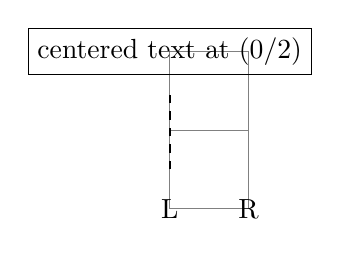
\begin{tikzpicture}
    % ~~~ help grid, from (0/0) to (1/2), 1 cm each ~~~~~~~
    \draw [help lines] (0,0) grid (1,2);
    % ~~~ placing a node, with text, draw its shape ~~~~~~~~
    \node [draw] at (0,2) {centered text at (0/2)};
    
    % Juan's special, simplified
    \foreach[count=\jj from 0]\j in {L,R} % left, right
    {
        \node at (\jj,0) {\j};  
    }
    
    % ~~~ just to emphasize placement ~~~~~~~~~~~~~~~~~~~
    \draw [dashed,thick] (0,.5) -- (0,1.5);

\end{tikzpicture}
\end{document}